\subsection{Psykologiske følger af fysisk inaktivitet}
Som nævnt i \autoref{sec:effekterafaktivitet} er fysisk inaktivitet en risikofaktor for visse psykiske lidelser. Eksempelvis er det påvist, at forekomsten af depression er lavere blandt fysisk aktive end blandt fysisk inaktive \citep{motionsraad2007}. Ud over depression er der nogen evidens for, at andre psykiske sygdomme såsom angst, misbrug, skizofreni og spiseforstyrrelser kan have gavn af større eller mindre mængde fysisk aktivitet i relation til sygdomsbehandlingen \citep{kessing2016}. Fysisk inaktivitet kan både have en rolle for sygdomsudviklingen samt den videre progredieren af sygdommen, hvor fysisk inaktivitet kan forværre symptomer og patientens generelle tilstand \citep{motionsraad2007,kessing2016}.

\subsubsection{Depression samt følelsesmæssig trivsel}
I studiet \citetalias{galper2006} af \citeauthor{galper2006}, undersøges sammenhængen mellem fysisk inaktivitet og depression samt følelsesmæssig trivsel. Forsøgspersonerne hertil blev delt op i grupper af inaktive, utilstrækkeligt aktive, tilstrækkeligt aktive og meget aktive, og disse grupper blev så vurderet, om de havde depressive symptomer, og om de trivedes følelsesmæssigt. 
Til dette benyttedes en skala, The General Well-Being Schedule (GWB), som dermed forsøger at kvantificere forsøgspersonernes følelsesmæssige trivsel samt en skala, Center for Epidemiologic Studies Depression Scale (CES-D), til at kvantificere depressive symptomer \citep{galper2006}.

\begin{figure}[H]
\centering
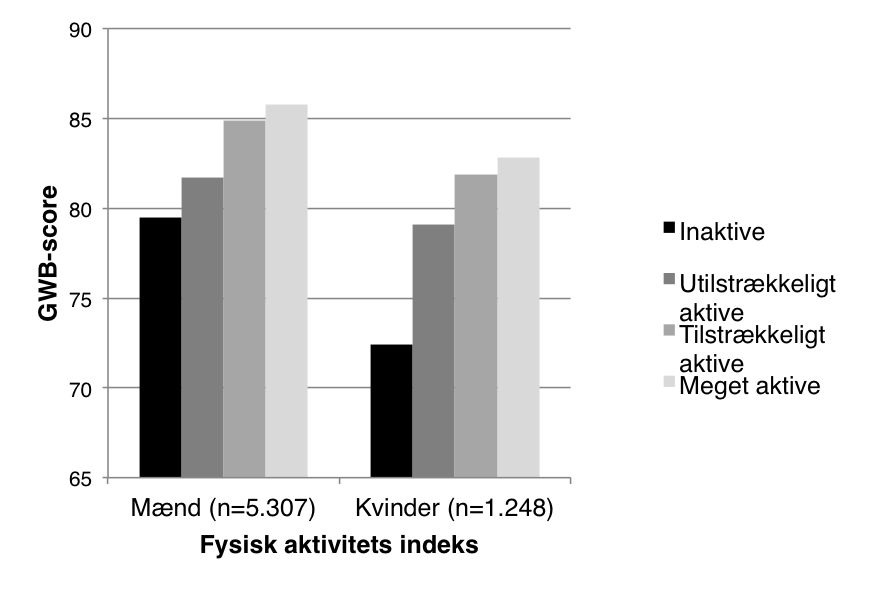
\includegraphics[width=0.6\textwidth]{figures/inaktivitet_gwb}
\caption{Fysisk inaktivitet sammenholdt med følelsesmæssig trivsel. På x-aksen fremgår grupperingen i fysisk aktivitetsniveau for henholdsvis mænd og kvinder. På y-aksen fremgår den gennemsnitlige GWB-score, hvilket indikerer følelsesmæssig trivsel på en skala fra $0-110$ \citep{galper2006}.}
\label{fig:inaktivitet_gwb}
\end{figure}

\begin{figure}[H]
\centering
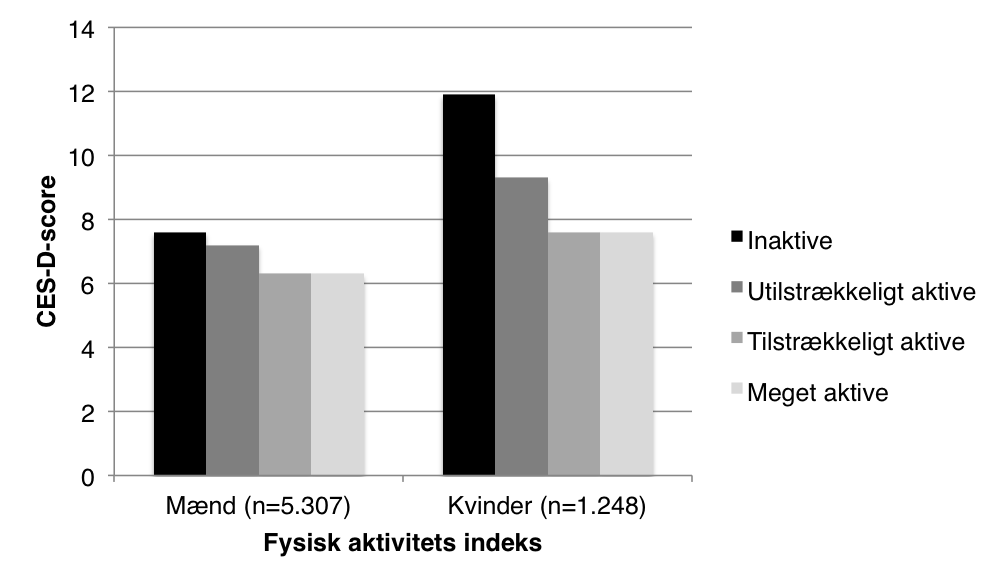
\includegraphics[width=0.6\textwidth]{figures/inaktivitet_dep}
\caption{Fysisk inaktivitet sammenholdt med depressionssymptomer. På x-aksen fremgår grupperingen i fysisk aktivitetsniveau for henholdsvis mænd og kvinder. På y-aksen fremgår den gennemsnitlige CES-D-score, hvilket indikerer depressive symptomer på en skala fra $0-60$ \citep{galper2006}.}
\label{fig:inaktivitet_dep}
\end{figure}

\noindent
Resultater herfra, som fremgår af \autoref{fig:inaktivitet_gwb} og \autoref{fig:inaktivitet_dep}, viser, at fysisk inaktive, især kvinder, har en højere tendens til depressive symptomer, end andre, der er mere fysisk aktive. På samme måde fremgik det af studiet, at fysisk inaktive forsøgspersoner  ikke trives følelsesmæssigt, sammenlignet med dem, der er mere aktive \citep{galper2006}. 

Studiet konkluderer derved, at der er en sammenhæng mellem fysisk inaktivitet og psykiske følger, som eksempelvis depression og forværret følelsesmæssig trivsel \citep{galper2006}. Yderligere er der evidens for, at fysisk inaktivitet forværrer allerede eksisterende depressionstilstande samt dårlig følelsesmæssig trivsel \citep{motionsraad2007}.
